%%%%%%%%%%%%%%%%%%%%%%%%%%%%%%%%%%%%%%%%%
% Structured General Purpose Assignment
% LaTeX Template
%
% This template has been downloaded from:
% http://www.latextemplates.com
%
% Original author:
% Ted Pavlic (http://www.tedpavlic.com)
%
% Note:
% The \lipsum[#] commands throughout this template generate dummy text
% to fill the template out. These commands should all be removed when
% writing assignment content.
%
%%%%%%%%%%%%%%%%%%%%%%%%%%%%%%%%%%%%%%%%%

%----------------------------------------------------------------------------------------
%	PACKAGES AND OTHER DOCUMENT CONFIGURATIONS
%----------------------------------------------------------------------------------------

% !TEX root = ./resumeDNA1.tex
\documentclass{article}

\usepackage{fancyhdr} % Required for custom headers
\usepackage{lastpage} % Required to determine the last page for the footer
\usepackage{extramarks} % Required for headers and footers
\usepackage{graphicx} % Required to insert images
\usepackage{lipsum} % Used for inserting dummy 'Lorem ipsum' text into the template
%% Packages used to read accented UTF-8 inputs
\usepackage[utf8]{inputenc}
\usepackage[T1]{fontenc}
% \usepackage{multicol} unused
% Packages for the Gantt diagram
\usepackage{pgfgantt}
\usepackage{xcolor}

% Margins
\topmargin=-0.45in
\evensidemargin=0in
\oddsidemargin=0in
\textwidth=6.5in
\textheight=9.0in
\headsep=0.25in

\linespread{1.1} % Line spacing

% Set up the header and footer
\pagestyle{fancy}
\lhead{\projAuthorName} % Top left header
\chead{\projName} % Top center header
\rhead{\date{01.10.2017}} % Top right header
\lfoot{\lastxmark} % Bottom left footer
\cfoot{} % Bottom center footer
\rfoot{Page\ \thepage\ of\ \pageref{LastPage}} % Bottom right footer
\renewcommand\headrulewidth{0.4pt} % Size of the header rule
\renewcommand\footrulewidth{0.4pt} % Size of the footer rule

\setlength\parindent{0pt} % Removes all indentation from paragraphs

%----------------------------------------------------------------------------------------
%	DOCUMENT STRUCTURE COMMANDS
%	Skip this unless you know what you're doing
%----------------------------------------------------------------------------------------

% Header and footer for when a page split occurs within a problem environment
\newcommand{\enterProblemHeader}[1]{
\nobreak\extramarks{#1}{#1 continued on next page\ldots}\nobreak
\nobreak\extramarks{#1 (continued)}{#1 continued on next page\ldots}\nobreak
}

% Header and footer for when a page split occurs between problem environments
\newcommand{\exitProblemHeader}[1]{
\nobreak\extramarks{#1 (continued)}{#1 continued on next page\ldots}\nobreak
\nobreak\extramarks{#1}{}\nobreak
}

\setcounter{secnumdepth}{0} % Removes default section numbers
\newcounter{homeworkProblemCounter} % Creates a counter to keep track of the number of problems

\newcommand{\homeworkProblemName}{}
\newenvironment{homeworkProblem}[1][Problem \arabic{homeworkProblemCounter}]{ % Makes a new environment called homeworkProblem which takes 1 argument (custom name) but the default is "Problem #"
\stepcounter{homeworkProblemCounter} % Increase counter for number of problems
\renewcommand{\homeworkProblemName}{#1} % Assign \homeworkProblemName the name of the problem
\section{\homeworkProblemName} % Make a section in the document with the custom problem count
\enterProblemHeader{\homeworkProblemName} % Header and footer within the environment
}{
\exitProblemHeader{\homeworkProblemName} % Header and footer after the environment
}

\newcommand{\problemAnswer}[1]{ % Defines the problem answer command with the content as the only argument
\noindent\framebox[\columnwidth][c]{\begin{minipage}{0.98\columnwidth}#1\end{minipage}} % Makes the box around the problem answer and puts the content inside
}

\newcommand{\homeworkSectionName}{}
\newenvironment{homeworkSection}[1]{ % New environment for sections within homework problems, takes 1 argument - the name of the section
\renewcommand{\homeworkSectionName}{#1} % Assign \homeworkSectionName to the name of the section from the environment argument
\subsection{\homeworkSectionName} % Make a subsection with the custom name of the subsection
\enterProblemHeader{\homeworkProblemName\ [\homeworkSectionName]} % Header and footer within the environment
}{
\enterProblemHeader{\homeworkProblemName} % Header and footer after the environment
}

%----------------------------------------------------------------------------------------
%	NAME AND TITLE SECTION
%----------------------------------------------------------------------------------------

\newcommand{\projName}{VisuDNA-II} % Assignment title
\newcommand{\projDate}{2017\textemdash2018}
\newcommand{\projAuthorName}{S. Bouquet} % Your name
\newcommand{\projSupervisors}{P. Kuonen, B. Wolf, J. Stoppani}
\newcommand{\projInitiator}{D. Atlan (PhenoSystem SA)}
\newcommand{\docTitle}{Resumé visuDNA}

%----------------------------------------------------------------------------------------
%	TITLE PAGE
%----------------------------------------------------------------------------------------

\title{
  
\includegraphics[width=0.9\columnwidth]{Logo_HEIA}\\
  \vspace{1cm}
  \textmd{\textit{Filière informatique}} \\
  \vspace{2cm}
  \textmd{Projet de semestre d'automne}\\
  \textmd{\projDate}\\
  \vspace{1.5cm}
  \noindent\makebox[\linewidth]{\rule{\textwidth}{0.5pt}}\\
  \vspace{.5cm}
  \textmd{\textbf{\projName}}\\
  \textmd{\textbf{\docTitle}}\\
  \noindent\makebox[\linewidth]{\rule{\textwidth}{0.5pt}}\\
  % \normalsize\vspace{0.1in}\small{\hmwkDueDate}\\
  % \vspace{0.1in}\large{\textit{\hmwkClassInstructor\ \hmwkClassTime}}
  \Large
  \vspace{3cm}
  \textit{Responsables:} \projSupervisors \\
  \vspace{1cm}
  \textit{Externe:} \projInitiator \\
  \vspace{1cm}
  \textit{Autheur:} \projAuthorName \\
  \author{}
}
% \author{\textbf{\projAuthorName}}
\date{} % Insert date here if you want it to appear below your name

%----------------------------------------------------------------------------------------

\begin{document}

\maketitle
%----------------------------------------------------------------------------------------
%	TABLE OF CONTENTS
%----------------------------------------------------------------------------------------

%\setcounter{tocdepth}{1} % Uncomment this line if you don't want subsections listed in the ToC

% \newpage
% \tableofcontents
 \newpage

%----------------------------------------------------------------------------------------
%	PROBLEM 1
%----------------------------------------------------------------------------------------

% To have just one problem per page, simply put a \clearpage after each problem

\section{Fonctionalités}
\subsection{UseCase}
Dans le but de bien comprendre le travail réaliser durant le précédent projet et dû au fait qu'aucun
diagramme d'utilisation de l'application générale n'était présent dans la documentation, une modélisation
du système existant (peut-être aproximative) a été réalisée.
\begin{figure}[!h]
  \center
  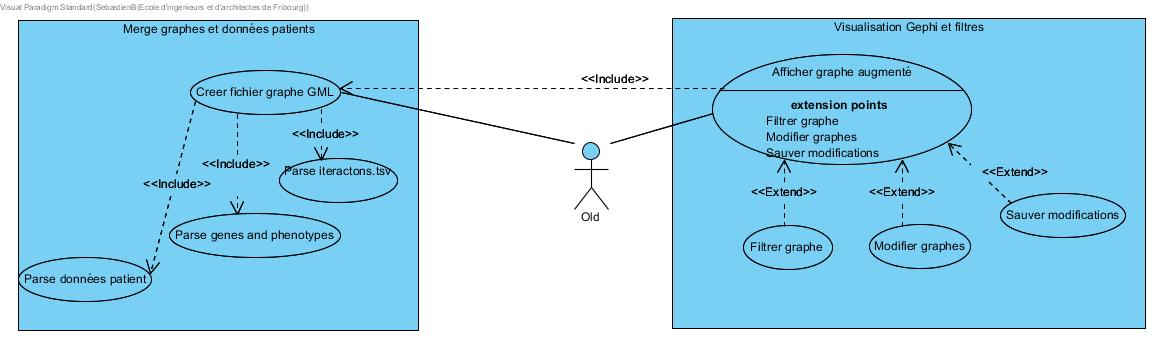
\includegraphics[width=\textwidth]{VisuDNA_UC}
  \caption{Diagramme d'utilisation du système existant}
\end{figure}

\subsection{Description}
On s'aperçoit que le projet est composé de deux parties: la première permettant de créer un fichier de graphe GML en associant les données de l'interactome avec les données du patient. On obtient ainsi un graphe augmenté qui peut être visualiser à l'aide de l'application Gephi.\\
La visualisation des graphes dans Gephi permet certaines option de filtre sur les graphes ainsi que l'ajout de modifications qui peuvent être sauvegardée dans le fichier de graphe.

\section{Choix de l'outil de visualisation}
\cite{Sisto:2015}
\subsection{Logiciels généraux de traitement de graphes}
L'état de l'art du projet précédent a révélé deux logiciels généraux qui semblaient convenir aux buts du projet car ils permettent le traitement de graphes conséquents et possèdent des plugins de traitement de graphes d'interactome. Il s'agissait de ``Cytoscape'' et de ``Gephi''. \\
\textit{A noté:} les plugins existants pour Cytoscape ne permettaient pas l'ajout d'annotation
sur les noeuds ni l'utilisation de sources de données autre que leur base de données
associée.
\subsection{Logiciels spécialisés}
Exemple de logiciels trouvés:
\begin{itemize}
  \item EINVis
  \item Navigator
  \item IGV
\end{itemize}
Ces outils ont reçus comme principale critique de ne pas permettre de grande liberté
quant à leur utilisation et au développement possible de modification.
\subsection{Séparer Gephi et cytoscape}
Ces deux outils ont les deux été retenus dans un premier temps car ils satisfont les critères suivants :
\begin{itemize}
  \item Traitement de gros graphes [sic].
  \item Possibilité de modifier le layout.
  \item Recherches personnalisée.
  \item Annotation personnalisée sour les noeuds et les arrêtes.
  \item Coloration des noeuds.
\end{itemize}
\textbf{Résultats:}\\
Le choix final du logiciel s'est fait sur les critères suivants. On s'aperçoit d'après
ces critères que ces deux logiciels sont relativement proches.
\begin{figure}[!h]
  \center
  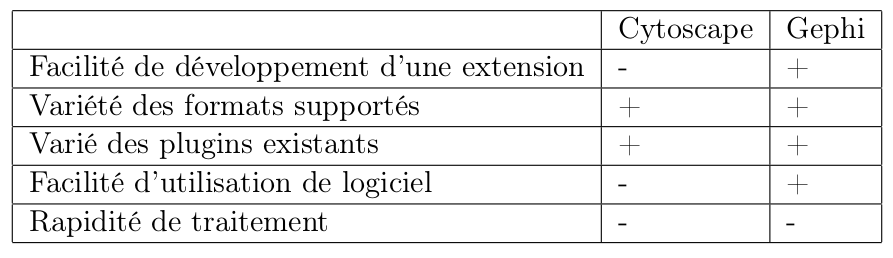
\includegraphics[width=10cm]{gephi_vs.png}
  \caption{Avantages Gephi vs Cytoscape}
\end{figure}
\subsection{Choix du format de graphe}
Le projet précédent a retenu le format GML car il semble simple et, surtout, il
est supporter par Gephi et Cytoscape.

%----------------------------------------------------------------------------------------

\newpage
\begingroup
  % Modifies the title of the "references" section
  \renewcommand{\section}[2]{\Large\textbf{Références}\normalsize}
  \bibliographystyle{model1-num-names}
  \bibliography{sample}
  \nocite{*}
\endgroup

\end{document}
